% \pagebreak[4]
% \hspace*{1cm}
% \pagebreak[4]
% \hspace*{1cm}
% \pagebreak[4]



\chapter{BraTS 2021 challenge and Kaggle leaderboard}
\ifpdf
    \graphicspath{{Kaggle/Chapter1Figs/PNG/}{Kaggle/Chapter1Figs/PDF/}{Kaggle/Chapter1Figs/}}
\else
    \graphicspath{{Kaggle/Chapter1Figs/EPS/}{Kaggle/Chapter1Figs/}}
\fi

% \begin{eqnarray}
% CIF: \hspace*{5mm}F_0^j(a) &=& \frac{1}{2\pi \iota} \oint_{\gamma} \frac{F_0^j(z)}{z - a} dz
% \end{eqnarray}



                              % first letter Z is for Acronyms 
% \nomenclature[aF]{$F$}{complex function}                                                   % first letter A is for Roman symbols
                                           % first letter G is for Greek Symbols
% \nomenclature[gi]{$\iota$}{unit imaginary number $\sqrt{-1}$}                      % first letter G is for Greek Symbols
% \nomenclature[gg]{$\gamma$}{a simply closed curve on a complex plane}  % first letter G is for Greek Symbols
% \nomenclature[xi]{$\oint_\gamma$}{integration around a curve $\gamma$} % first letter X is for Other Symbols

% first letter R is for superscripts                                                        % first letter S is for subscripts




The Radiological Society of North America (RSNA) teamed up with the Medical Image Computing and Computer Assisted Intervention Society (MICCAI) to improve the treatment planning for patients with glioblastoma. The RSNA-ASNR-MICCAI BraTS 2021
challenge (\cite{Brats}) targetted the evaluation of ML algorithms assessing
the tumour region segmentation, as well as the underlying tumor’s molecular characterization, in pre-operative baseline MRI imaging data. Specifically, the two tasks that BraTS 2021 focuses on are: a) the segmentation of the histologically distinct brain tumor sub-
regions, and b) the classification of the tumor’s O[6]-methylguanine-DNA
methyltransferase (MGMT) promoter methylation status. 

\vspace*{3mm} 
 The part 2 of the competition which involves predicting the MGMT methylation status of the given patient MRI smaples was hosted on Kaggle\footnote{\href{https://www.kaggle.com/competitions/rsna-miccai-brain-tumor-radiogenomic-classification}{https://www.kaggle.com/competitions/rsna-miccai-brain-tumor-radiogenomic-classification}}. Kaggle is an online community of data scientists and machine learning practitioners.
\vspace*{8mm}

\hypersetup{ colorlinks=true,
    linkcolor=black,
    filecolor=magenta,      
    urlcolor=blue}

\section{Current Kaggle leaderboard}
% \begin{figure}[!htbp]
%   \begin{center}
%     \leavevmode
%     \ifpdf
%       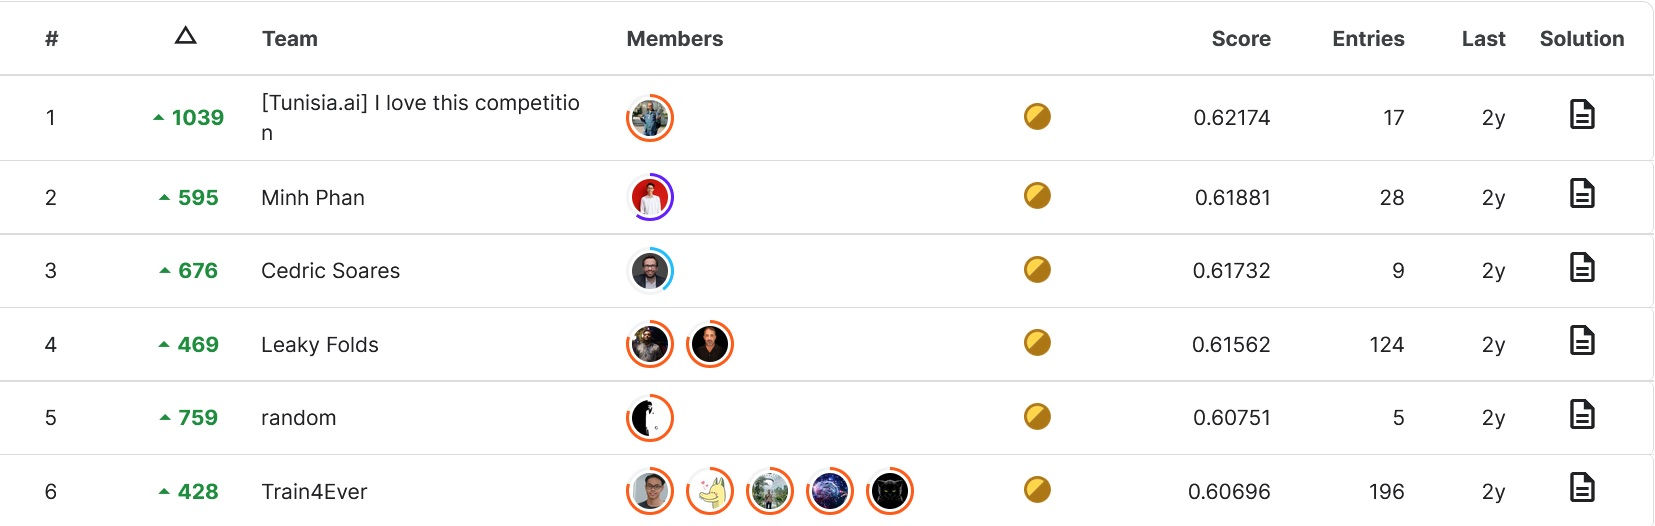
\includegraphics[height=2in]{Kaggle_leaderboard}
%     \else
%       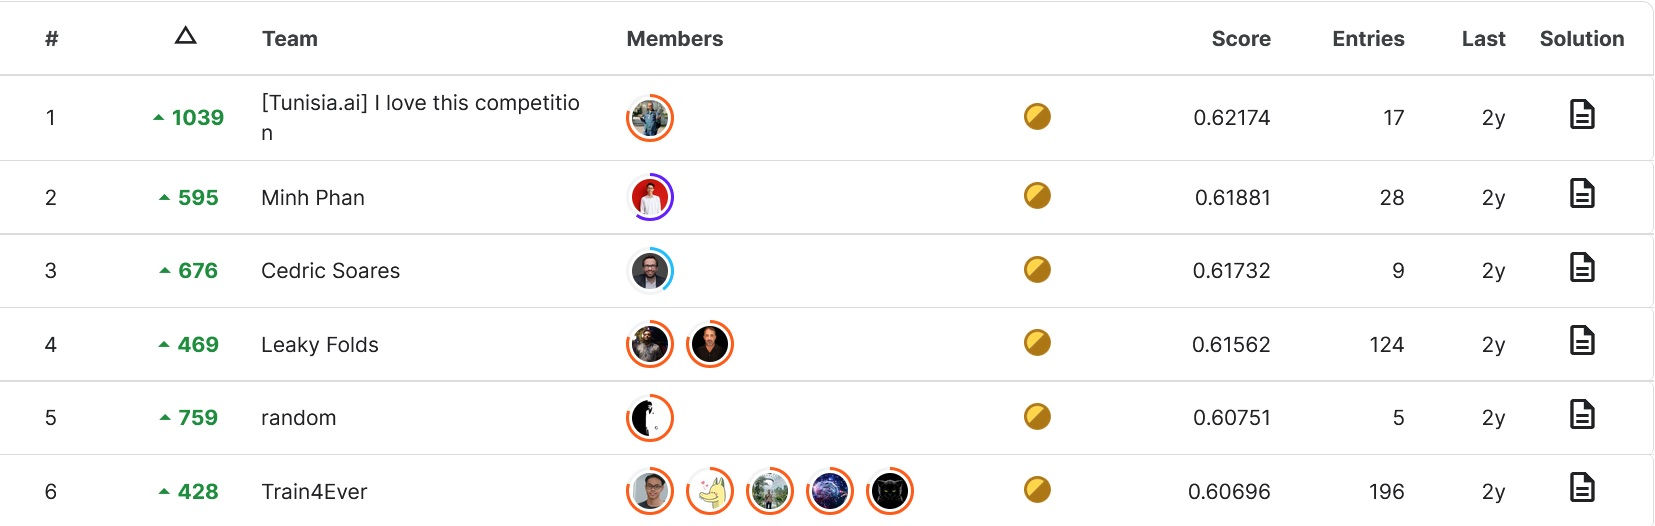
\includegraphics[bb = 92 86 545 742, height=6in]{Kaggle_leaderboard}
%     \fi
%     \caption{Kaggle leaderboard Top 6 teams}
%     \label{FigKaggleLeaderboard}
%   \end{center}
% \end{figure}
The Kaggle 2021 competition saw the participation of 1555 teams. The following table summarizes the model architectures and scores of the top six teams of the currently featuring \href{https://www.kaggle.com/competitions/rsna-miccai-brain-tumor-radiogenomic-classification/leaderboard}{leaderboard}. 

\vspace*{6mm}
\begin{table}[h!]
\centering
\begin{tabular}{ p{2cm} p{5.5cm} p{4cm}  }
 \hline
 \multicolumn{3}{c}{\thead{Current BraTS 2021 leaderboard}} \\
 [0.8ex]
 \hline
  \thead{Rank} & \thead{Model used} & \thead{AUC performance} \\  [0.8ex]
 \hline
 1   & 3D CNN + ResNet    & 0.621 \\  [0.8ex]
 2 &   EfficientNet + LSTM  & 0.618   \\  [0.8ex]
 3 & 4 parallel EfficientNet & 0.617  \\  [0.8ex]
 4 & YOLO (2D) + 3D CNN & 0.615 \\  [0.8ex]
 5 &   EfficientNet  & 0.607 \\  [0.8ex]
 6 & UNet + LSTM  & 0.606 \\  [0.8ex]
 \hline
\end{tabular}
\caption{Kaggle leaderboard top 6 teams}
\label{table:1}
\end{table}

\vspace*{6mm}

The \textbf{Rank 1} team uses a combination of 3D CNNs and a popular ResNet architecture to stack the 2D scans around an appropriately chosen 2D middle slice (from given DCM files) and then pass the 3D volume for classification. 3D CNNs are computationally exhaustive and require a heavy GPU for the larger convolutional load. The \textbf{Rank 2} team uses a complex sampling stretegy to introduce sequentiality into the data. They sample 10 scans from all patients (uniform temporal subsampling) across the 4 MRI modalities (T1cE, T2cE, T1wCE, Flair) to get 4-slice stacks which were fed into an LSTM network. 

\vspace*{3mm}

The \textbf{Rank 3} team uses 4 EfficientNet networks parallely for each of the 4 given modalities. The networks are simulatenously trained during the training phase, but in the testing phase, for each modality, predictions are obtained on a slice-by-slice basis and the most confident prediction probability is selected. Finally on the patient level, the average across 4 modality is obtained. The \textbf{Rank 4} team uses YOLO models on the 2D slices to detect the slices which have the best tumour visibility and then feed them into pre-trained classification networks. The \textbf{Rank 5} team sampled 10 images from each modality (patient level), took pixel intensity average of the 10 images to obtain one single image per modality, then stacked them together to get 4-slice-stacks. It was then fed to an EfficientNet model. Lastly, the \textbf{Rank 6} team sampled 2D slices from segmentation masks (with high tumour visibility) to get 2 masks (Tumour core, Enhancing tumour). The 2D slice was stacked with 2 kinds of mask to get 3-slice input, which was then fed to an LSTM network in chunks. 



\vspace*{6mm}

\hypersetup{ colorlinks=true,
    linkcolor=black,
    filecolor=magenta,      
    urlcolor=black}

\section{Observations and Scope}

The leaderboard test dataset AUCs saturate at around 0.61.
Observing the leaderboard approaches, it can be sensed that less focus is being given to localize the tumour voxel and then feed the Region-of-interest into a suitable classification network. Hence, the utility of an efficient Tumour segmentation task becomes apparent. Localization of the tumour region can be done in 2D slice basis or by taking into account the whole 3D volume. In this report, we highlight our investigations in this direction.  
\vspace{3mm}

It is to be noted that the tumour segmentation and Multi-task model based experiments was conducted in the Autumn semester (Sem 1 2022-23) while the volumetric projections and cropped-cascaded model tests were conducted in the Spring semester (Sem 2 2022-23). The source code, implementations, models can be found in the GitHub\footnote{\href{https://github.com/Deepan2486/Radiogenomic-classification-glioblastoma-multimodal-3D-MRI}{https://github.com/Deepan2486/Radiogenomic-classification-glioblastoma-multimodal-3D-MRI}} repository.
% \cite{texbook}

% \subsection{sub first paragraph}
% ... and some more ...



% above code has been macro-fied in Classes/MacroFile.tex file
%\InsertFig{\IncludeGraphicsH{aflow}{6in}{92 86 545 742}}{Airfoil Picture}{FigAir}

% So as we have now labelled it we can reference it, like so (\ref{FigKaggleLeaderboard}) and it
% is on Page \pageref{FigKaggleLeaderboard}. And as we can see, it is a very nice picture and we
% can talk about it all we want and when we are tired we can move on to the next
% chapter ...

\ifpdf
  \pdfbookmark[2]{bookmark text is here}{And this is what I want bookmarked}
\fi
% ------------------------------------------------------------------------


%%% Local Variables: 
%%% mode: latex
%%% TeX-master: "../thesis"
%%% End: 
